%% LyX 2.3.6.2 created this file.  For more info, see http://www.lyx.org/.
%% Do not edit unless you really know what you are doing.
\documentclass[english]{article}
\usepackage[T1]{fontenc}
\usepackage[latin9]{inputenc}
\pagestyle{plain}
\setcounter{secnumdepth}{0}
\usepackage{float}
\usepackage{amsmath}
\usepackage{amssymb}
\usepackage{graphicx}

\makeatletter
%%%%%%%%%%%%%%%%%%%%%%%%%%%%%% User specified LaTeX commands.


%%%%%%%%%%%%%%%%%%%%%%%%%%%%%%%%%%%%%%%%%%%%%%%%%%%%%%%%%%%%%%%%%%%%%%%%%%%%%%%%%%%%%%%%%%%%%%%%%%%%%%%%%%%%%%%%%%%%%%%%%%%%%%%%%%%%%%%%%%%%%%%%%%%%%%%%%%%%%%%%%%%%%%%%%%%%%%%%%%%%%%%%%%%%%%%%%%%%%%%%%%%%%%%%%%%%%%%%%%%%%%%%%%%%%%%%%%%%%%%%%%%%%%%%%%%%
\usepackage{amsfonts}

\setcounter{MaxMatrixCols}{10}
%TCIDATA{TCIstyle=LaTeX article (bright).cst}

%TCIDATA{OutputFilter=LATEX.DLL}
%TCIDATA{Version=5.00.0.2606}
%TCIDATA{<META NAME="SaveForMode" CONTENT="1">}
%TCIDATA{BibliographyScheme=Manual}
%TCIDATA{Created=Thursday, September 13, 2001 12:48:34}
%TCIDATA{LastRevised=Friday, April 28, 2006 16:52:00}
%TCIDATA{<META NAME="GraphicsSave" CONTENT="32">}
%TCIDATA{<META NAME="DocumentShell" CONTENT="Exams and Syllabi\SW\Assignment">}
%TCIDATA{Language=American English}

\setlength{\topmargin}{-1.0in}
\setlength{\textheight}{9.25in}
\setlength{\oddsidemargin}{0.0in}
\setlength{\evensidemargin}{0.0in}
\setlength{\textwidth}{6.5in}
\def\labelenumi{\arabic{enumi}.}
\def\theenumi{\arabic{enumi}}
\def\labelenumii{(\alph{enumii})}
\def\theenumii{\alph{enumii}}
\def\p@enumii{\theenumi.}
\def\labelenumiii{\arabic{enumiii}.}
\def\theenumiii{\arabic{enumiii}}
\def\p@enumiii{(\theenumi)(\theenumii)}
\def\labelenumiv{\arabic{enumiv}.}
\def\theenumiv{\arabic{enumiv}}
\def\p@enumiv{\p@enumiii.\theenumiii}


\parindent=0pt

\makeatother

\usepackage{babel}
\begin{document}
\begin{center}
\textbf{Written Exam for Nonlinear Dynamics and Chaos II, Spring Semester,
2013}
\par\end{center}

\begin{center}
August 20, 2013;9:00-10:00am, ML F36\emph{. Use of class-notes (hand-written
or printed copy) is allowed}
\par\end{center}

\bigskip{}

Thermohaline circulation (THC) is a part of the large-scale ocean
circulation that is driven by global density gradients created by
surface heat and freshwater fluxes. Stommel's box model (1961) is
a qualitative description of the trends and equilibria in THC. This
model couples the two fundamental drivers of TLC, temperature (\emph{thermo})
and salt concentration (\emph{-haline}), in a nonlinear fashion.

\begin{center}
\begin{figure}[H]
\centering{}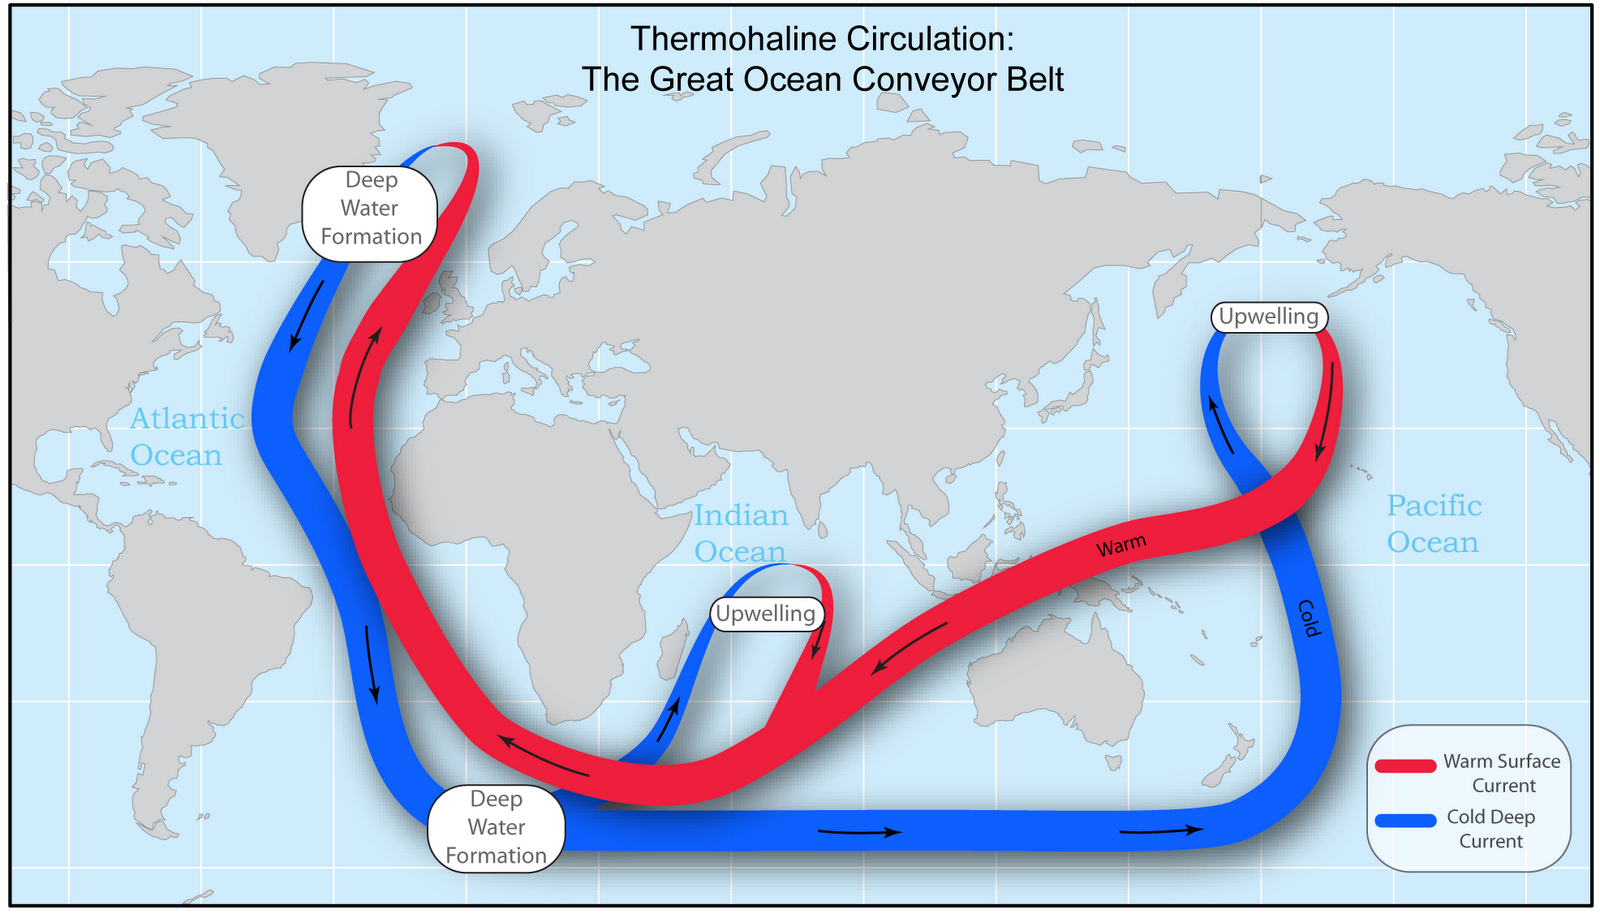
\includegraphics[width=0.7\textwidth]{thermohaline}
\end{figure}
\par\end{center}

The non-dimensional \textbf{variables} of Stommel's model are:

~~
\begin{description}
\item [{$x(t)$:}] temperature difference between the tropics (lower latitudes)
and the North-Atlantic (higher latitudes)
\item [{$y(t)$:}] salinity (i..e, salt concentration) difference between
the above two regions of the ocean
\item [{~~}]~
\end{description}
The non-dimensional \textbf{parameters} of the model are:

~~
\begin{description}
\item [{$\tau_{x}$:}] relaxation time to a constant temperature difference
between northern and southern latitudes in the absence of coupling
\item [{$\tau_{y}$:}] relaxation time to zero salinity difference between
higher and lower latitudes in the absence of coupling. In practice,
$\tau_{x}/\tau_{y}=\epsilon\ll1.$
\item [{$\mu$:}] measure of freshwater flux through clouds moving from
lower to higher latitudes
\item [{$\eta:$}] nonlinear coupling parameter between temperature and
salinity evolution
\end{description}
With this notation, Stommel's model can be written as
\begin{align*}
\dot{x} & =-\frac{1}{\tau_{x}}(x-1)+\frac{1}{\tau_{y}}x\left[1+\eta^{2}(x-y)^{2}\right],\\
\dot{y} & =\frac{\mu}{\tau_{y}}-\frac{1}{\tau_{y}}y\left[1+\eta^{2}(x-y)^{2}\right].
\end{align*}

\begin{enumerate}
\item Show that Stommel's model has a globally attracting slow manifold
that governs the asymptotic behavior of THC. Find a leading order
approximation to this manifold. (\emph{Hint}: rescale time by letting
$s=t/\tau_{y}.)$
\item Compute the leading-order reduced flow on the slow manifold. Determine
qualitatively the possible dynamical behaviors on the slow manifold
as the parameters $\mu$ and $\eta$ are varied.
\end{enumerate}

\end{document}
